% Copyright (C) 2005-2015 Airbus - EDF - IMACS - Phimeca
% Permission is granted to copy, distribute and/or modify this document
% under the terms of the GNU Free Documentation License, Version 1.2
% or any later version published by the Free Software Foundation;
% with no Invariant Sections, no Front-Cover Texts, and no Back-Cover
% Texts.  A copy of the license is included in the section entitled "GNU
% Free Documentation License".
\renewcommand{\filename}{docUC_StocProc_NonStationaryCovarianceFunction_UserDefined.tex}
\renewcommand{\filetitle}{UC : Creation of a User defined covariance function}

% \HeaderNNIILevel
% \HeaderIILevel
\HeaderIIILevel

\label{CovarianceModelCreation}
\index{Stochastic Process!Covariance Model}

This use case illustrates how the User can define his own covariance model.\\

A covariance function $C$ is defined by : $C : \cD \times \cD \rightarrow \mathbb{M}_{d \times d}(\Rset)$ where $C(\vect{s}, \vect{t})$ is a covariance matrix of dimension~$d$.\\
The domaine $\cD$ is discretized on the mesh $\cM$.\\


OpenTURNS allows the User to define his own covariance model thanks to the object {\itshape UserDefinedCovarianceModel} defined from :
\begin{itemize}
\item a mesh $\cM \in \Rset^n$ defined by the vertices $(\vect{t}_0,\dots, \vect{t}_{N-1})$ and the associated simplices,
\item a collection of $N(N+1)/2$ covariance matrices stored in the object \emph{CovarianceMatrixCollection} noted $(\mat{C}_{k,\ell})_{0 \leq \ell \leq k \leq N-1}$ where $\mat{C}_{k,\ell} \in \mathcal{M}_{d \times d}(\Rset)$.\\

  Care: The covariance matrices $(\mat{C}_{i,j})_{0 \leq j \leq i \leq N-1}$ must be given in the following order:
  \begin{align*}
    \mat{C}_{0,0}, \, \mat{C}_{1, 0}, \, \mat{C}_{1,1}, \, \mat{C}_{2,0},  \,\mat{C}_{2,1},\, \mat{C}_{2,2}, \,\dots
  \end{align*}
  which corresponds to the global covariance matrix, which lower part is:
  \begin{align*}
    \left(
    \begin{array}{cccc}
      \mat{C}_{0,0}& & & \\
      \mat{C}_{1,0}&  \mat{C}_{1,1}& & \\
      \mat{C}_{2,0}&   \mat{C}_{2,1}& \mat{C}_{2,2}& \\
      \dots & \dots & \dots & \dots
    \end{array}
    \right)
  \end{align*}
\end{itemize}


Using that collection of covariance matrices, OpenTURNS builds a covariance function which is a  piecewise constant function defined on $\cD \times \cD$ by:
\begin{align*}
  \forall (\vect{s}, \vect{t}) \in \cD \times \cD, \, \quad C(\vect{s}, \vect{t}) =  \mat{C}_{k(\vect{s}),k(\vect{t})}
\end{align*}
where $k(\vect{s})$ is such that $\vect{t}_{k(\vect{s})}$ is the  vertex of $\cM$ the nearest to $\vect{s}$.\\
It follows that:
\begin{align*}
  C(\vect{t}_k, \vect{t}_\ell) = \mat{C}_{k,\ell}
\end{align*}
Concerning the  collection of covariance matrices that is used to build the discretized covariance model, we have that:
\begin{itemize}
\item the  matrix $\mat{C}_{k,\ell}$ has the index $n=\ell +\dfrac{k(k+1)}{2}$.
\item inversely, the matrix stored at index $n$ in the collection of covariance matrices, is the matrix $\mat{C}_{k,\ell}$ where:
  \begin{align*}
    k=\left\lfloor \dfrac{1}{2}\left( \sqrt{8n+1}-1 \right) \right\rfloor
  \end{align*}
  and
  \begin{align*}
    \ell= n-\dfrac{k(k+1)}{2}
  \end{align*}
\end{itemize}




\requirements{

  \begin{description}
  \item[$\bullet$] a mesh : {\itshape myMesh}
  \item[type:]  Mesh
  \end{description}

  \begin{description}
  \item[$\bullet$] a collection of covariance matrices : {\itshape myCovarianceCollection}
  \item[type:]  CovarianceMatrixCollection
  \end{description}

  \begin{description}
  \item[$\bullet$] two vertices : {\itshape s,t}
  \item[type:]  NumericalPoint
  \end{description}

}
{
  \begin{description}
  \item[$\bullet$] a covariance model : {\itshape myCovarianceModel}
  \item[type:] UserDefinedCovarianceModel
  \end{description}

}

\textspace\\
Python script for this UseCase :

\inputscript{script_docUC_StocProc_NonStationaryCovarianceFunction_UserDefined}

\textspace\\


In the following example, we illustrate the piecewise constant covariance that OpenTURNS builds from a collection of covariance matrices that comes from the continuous covariance function $C : \cD \times \cD \rightarrow  \Rset $ defined by:
\begin{align}
  \displaystyle C(s,t) = \exp\left(-\dfrac{4|s-t|}{1+s^2+t^2}\right)
\end{align}
where  the domain $\cD=[-4,4]$ discretized on the mesh $\cM$ which is the regular time grid with $N=64$ points: $(t_0, \dots, t_{63})$.\\
As we have $n=1$ and $d=1$, the covariance matrices are scalars and the colelction corresponds to  $(C(t_i,t_j))_{0 \leq j \leq i \leq 63}$.\\

The Figure \ref{UserDefinedNonStationaryCovarianceModelDemonstration} draws the iso contours of the continuous model $C$ and the piecewise constant model built by OpenTURNS: the discretized models approaches the real one with a good precision.


\begin{figure}[H]
  \begin{center}
    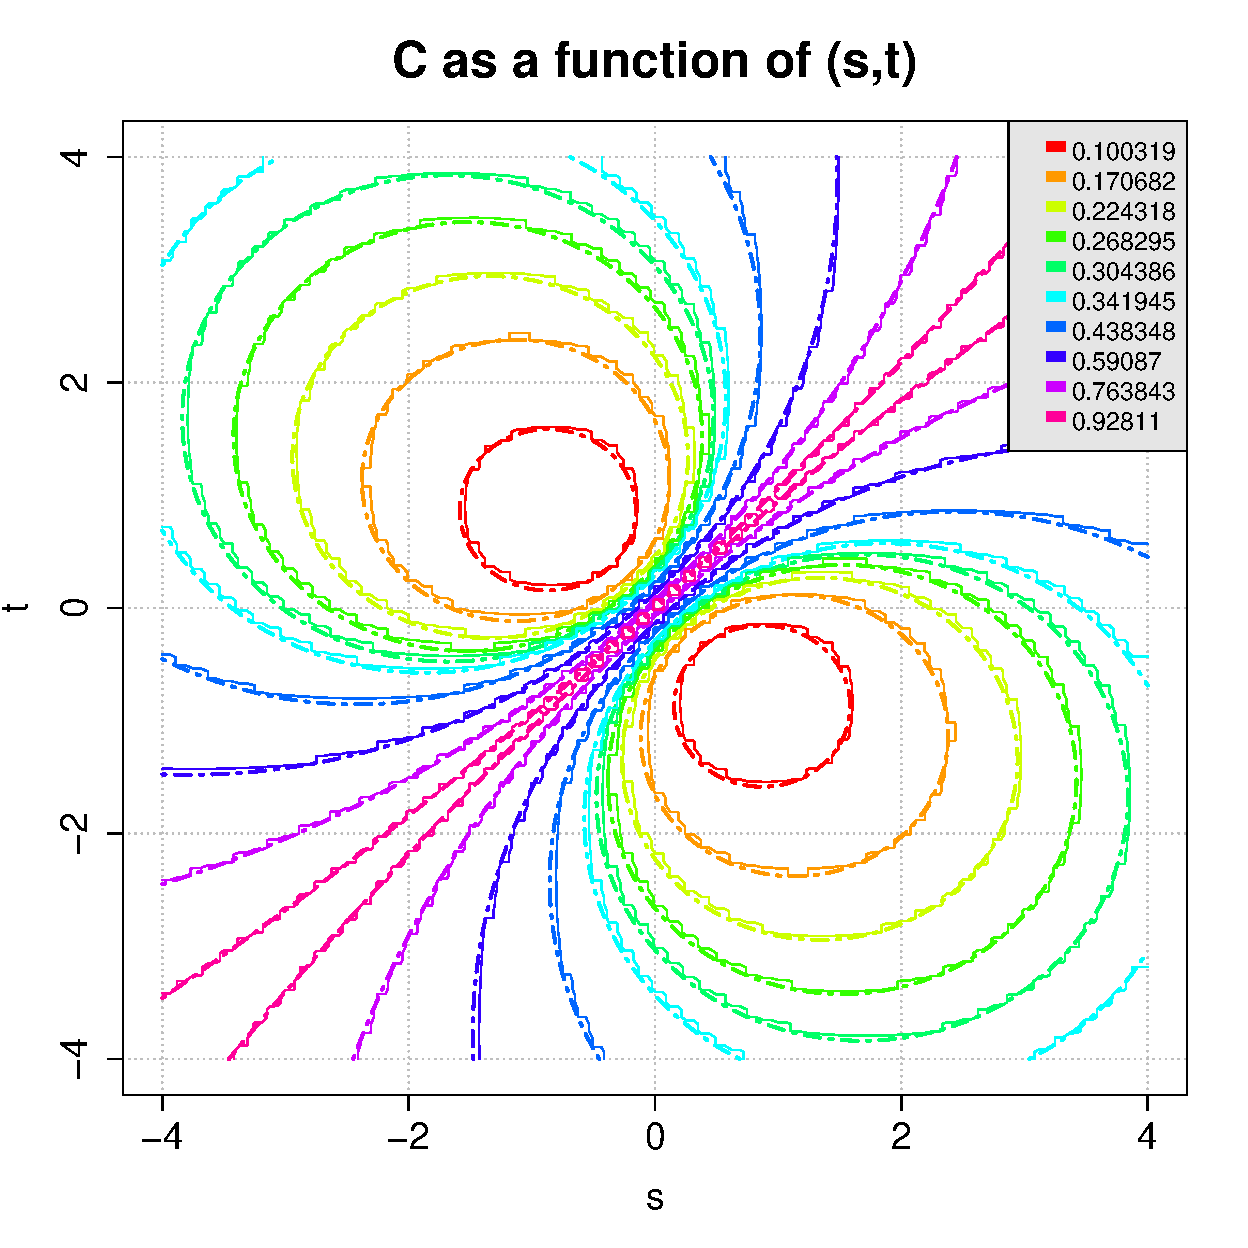
\includegraphics[width=7cm]{Figures/NonStationCovFunc.pdf}
    \caption{User defined non stationary covariance model in dimension 1 on $\cD=[-4,4]$.}
    \label{UserDefinedNonStationaryCovarianceModelDemonstration}
  \end{center}
\end{figure}
